\section{Implementation}\label{sec:implementation}

The compiler \code{orchc} is about 7,900 lines of C++17 with no dependencies
(\cref{fig:pipeline}). A recursive-descent parser with error recovery feeds a
semantic analysis that assigns binding identities and computes both labels of every
value. The cost analysis derives the output bound, the estimated input and the
guaranteed input of \cref{sec:bounds}; the relational analysis computes signatures,
resolves secret branches and checks the leakage budget. The two withdrawn rules of
\cref{sec:failed} remain in the code base as selectable baselines
(\code{--relational-rule bounds|sizes}), so that the evaluation can run all three on
the same workflows. The certificate emitter writes the JSON certificate of
\cref{sec:language}, which records the analysis version, the relational rule used and
the SHA-256 digest of the source. \code{make check} builds with
\code{-Wall -Wextra -pedantic} and runs 137 tests, among them every counterexample
from both audits.

\begin{figure}[t]
\centering
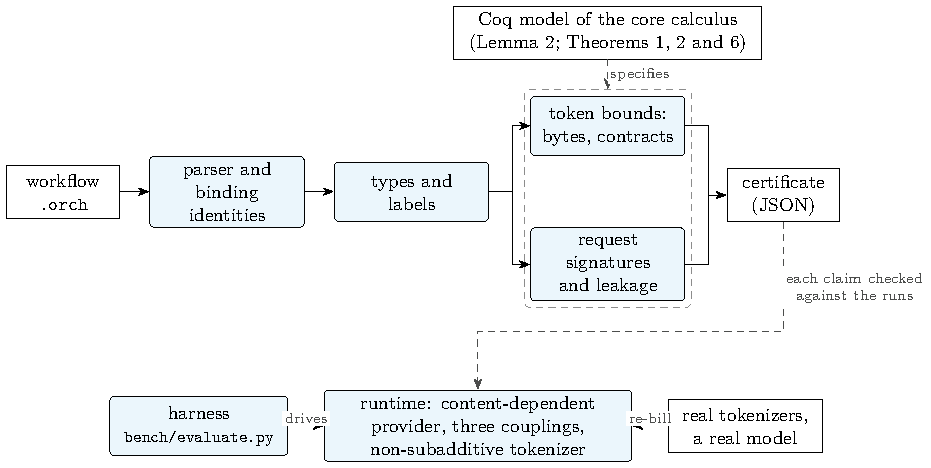
\includegraphics[width=\textwidth]{fig-pipeline.pdf}
\caption{Architecture. The compiler checks a workflow in three stages and emits a
certificate; the harness then runs every workflow under the mock runtime and checks each
claim of the certificate against the runs, re-billing requests with real tokenizers. The Coq
model specifies the two analyses for the core calculus but is not connected to the C++ code.
(Diagram drawn in TikZ with the help of Claude, Anthropic.)}
\label{fig:pipeline}
\end{figure}

\paragraph{A runtime built to falsify the analyses} The first version of the
runtime shared the blind spot of the rule it was meant to test. It drew every output
length uniformly at random, whatever the request said, and billed input with the
analysis's own estimate. Those are exactly the assumptions under which comparing
sizes is sound, so that runtime could not have revealed the failures of
\cref{sec:failed}. The current runtime has a content-dependent provider mode, in
which each draw is mixed with a hash of the request, so any change to a request
changes the answer. Its mock tokenizer uses greedy longest match over a small
vocabulary with overlapping entries, so it is not subadditive, as real tokenizers are
not. It implements the three keying schemes of \cref{sec:couplings}, and it bills
per model name as a provider's invoice would. With \code{run --json} it emits the
full transcript, which is what the harness compares.

\paragraph{The harness} The script \file{bench/evaluate.py} checks every relational
verdict under every combination of provider mode, keying scheme and accounting mode,
re-bills recorded requests with real tokenizers, and exits with a nonzero status on
any violation of a certificate. It too was rewritten: an earlier version skipped
failing cases, counted any nonzero exit of the compiler as a detected leak, and
returned success despite recorded violations. A harness that cannot fail cannot
support a claim, so we tested checks by breaking the property they check; for
instance, the check that a ported prompt occurs in its source was run against a port
into which we had inserted an invented sentence, and it failed as it should.

\paragraph{How the artifact was produced} The compiler, the harness and the Coq
development were written with the help of an AI coding assistant (Claude,
Anthropic), working under the author's direction. We report this here because it
concerns the method: none of the results depends on trusting that process, since
each is reproduced by the artifact's own checks (\code{make check}, \code{make proofs}
and \code{python bench/evaluate.py}), and \cref{sec:evaluation} reports what those
checks print.
